\documentclass[conference]{IEEEtran}
%\IEEEoverridecommandlockouts
% The preceding line is only needed to identify funding in the first footnote. If that is unneeded, please comment it out.
\usepackage{cite}
\usepackage{amsmath,amssymb,amsfonts}
\usepackage{algorithmic}
\usepackage{graphicx}
\usepackage{textcomp}
\usepackage[table]{xcolor}
\usepackage{url}
\usepackage{hyperref}
%\usepackage{subcaption}
%\usepackage{subfig}
\usepackage{array}
\usepackage{multirow}
\usepackage{multicol}
\hypersetup{
    colorlinks = true,
    linkcolor = blue,
    anchorcolor = blue,
    citecolor = blue,
    filecolor = blue,
    urlcolor = blue
}	
\usepackage[ruled,vlined]{algorithm2e}
\newcommand\MyBox[2]{
    \fbox{\lower0.75cm
        \vbox to 1.7cm{\vfil
            \hbox to 1.7cm{\hfil\parbox{1.4cm}{#1\\#2}\hfil}
            \vfil}%
    }%
}

\def\BibTeX{{\rm B\kern-.05em{\sc i\kern-.025em b}\kern-.08em
        T\kern-.1667em\lower.7ex\hbox{E}\kern-.125emX}}
\begin{document}
    \title{Comparing Parallel Sorting Algorithms on a High Performance Computing Cluster Using OpenMP}
    \author{\IEEEauthorblockN{Benjamin Pierce\\\href{mailto:bgp12@case.edu}{bgp12@case.edu}}
        \IEEEauthorblockA{
            \textit{Department of Computer and Data Sciences}\\ }
        \and
        \IEEEauthorblockN{Alberto Safra\\\href{mailto:axs1249@case.edu}{axs1249@case.edu}}
        \IEEEauthorblockA{ 
	    \textit{NCDP, Dean's Deptartment}}
        \and
        \IEEEauthorblockN{Colin Causey\\\href{mailto:cjc158@case.edu}{cjc158@case.edu}}
        \IEEEauthorblockA{ 
            \textit{Department of Computer and Data Sciences}}
        \and
        \IEEEauthorblockN{Jason Richards\\\href{mailto:jdr145@case.edu}{jdr145@case.edu}}
        \IEEEauthorblockA{
            \textit{Department of Computer and Data Sciences}}}
    \maketitle
    
    \begin{abstract}
        Sorting is commonly viewed as the most fundamental problem in the study of algorithms. Some cited reasons for this are that a great many software applications use sorting for various reasons, and a great many algorithms use sorting as a subroutine \cite{cormen_introduction_2009}. 
        Given sorting's ubiquity, therefore, it is valuable to be able to solve the sorting problem efficiently. 
        For this reason, many efficient sorting algorithms have been developed and studied. Three of the most popular and efficient sorting algorithms are Mergesort, Quicksort,  and Heapsort. 
        Given the asymptotic lower bound of $\Omega(nlog(n))$ for comparison-based sorting algorithms such as these, a natural route to take to achieve greater performance is parallel computing. 
        In the interest of wanting to select the optimal sorting algorithm to run on a particular parallel computing architecture, it is valuable to empirically compare the performance of different parallelized sorting algorithms. 
        This is the aim of our research. 
        In this project, we conduct an empirical analysis and comparison of parallelized versions of two popular sorting algorithms: Mergesort and Quicksort. Heapsort and the difficulties of parallelizing it are also considered. 
        The criteria for evaluation are (i) execution time and (ii) scalability. 
        The research was conducted on Case Western Reserve’s high-performance computing (HPC) architecture, specifically the Markov cluster. 
        We implement parallel Mergesort and Quicksort and execute them with variously sized and randomly permuted input arrays. The execution times are recorded for each run. 
        Additionally, we run the algorithms on a varying number of CPUs (e.g., one CPU, two CPUs, four CPUs) in order to assess their scalability.
        After collecting the data, we perform data analysis and use it to compare the algorithms according to the aforementioned criteria for evaluation. 
        The comparison will facilitate making an informed choice about which sorting algorithm to use under various conditions (e.g., the number of CPUs available and the size of the input array).
    \end{abstract}
    
    \section{Introduction}
    Sorting is a fundamental problem to be solved in many algorithms and applications.
    Any algorithm or application, for instance, that depends on having some ordering to its data will likely deal with sorting in some form. Because of its pervasiveness, solving the sorting problem efficiently is highly desirable. For this reason, many efficient sorting algorithms have been developed. Three of the most popular are Mergesort, Quicksort, and Heapsort. All three of these algorithms have time complexities of $O(nlog(n))$ in the average case. Mergesort and Heapsort also achieve this time bound in the worst case, while Quicksort can in rare situations exhibit a runtime of $O(n^2)$ in the worst case. Since the asymptotic lower bound for comparison-based sorting algorithms such as these is $\Omega(nlog(n))$, significantly improving the performance of them isn't feasible with serial computation. For this reason, we must turn to parallel computation to achieve significant performance gains. In order to take advantage of the performance increases enabled by parallel computing, parallelized versions of various sorting algorithms have been developed and studied. While theoretical analysis of parallel sorting algorithms is useful for understanding the asymptotic differences in the runtimes, determining and analysing the empirical performance of the algorithms on a specific computer architecture is valuable for making an informed choice about which algorithm to choose for that particular architecture and under various conditions (e.g., the number of CPUs available and the size of the input array to sort).
    This study focuses on an empirical evaluation of parallelized versions of two of the most popular sorting algorithms: Mergesort and Quicksort. Heapsort is also analyzed as it is comparable to Mergesort and Quicksort, although it is not parallelized due to difficulties that we will discuss. Instead, it is used as a reference serial algorithm to compare against our two parallelized algorithms. The algorithms are parallelized with OpenMP so as to take advantage of multithreaded, shared-memory parallelism on Case Western Reserve University's HPC Markov cluster. The criteria for evaluation are (i) execution time and (ii) scalability, i.e., the extent to which adding more processors decreases execution time.

\indent The layout of the paper is as follows: In Section II, we give an overview of parallel computing and the sorting algorithms that are included in our experiment and analysis. In Section III, we lay out our experimental methodology for comparing our sorting algorithms. Section IV presents our results and analysis. In Section V, we give our concluding remarks. Finally, in the Appendix, we provide information for how to access our code and data and how to run our experiment on the Case Western Markov cluster. % Weird space
    
    \section{Background \& Theory}
    Today's world of "Big Data" has led to an astronomical increase in the amount of computing power needed to efficiently process data.
    As a result, parallel computing has become an important and necessary approach to solving computationally-intensive problems.
    Parallel computing is a paradigm where computation is spread across many processors working on multiple tasks and/or data at the same time. This is in contrast to serial computation in which each step of a computation is performed one after another.
    The processors used in parallel computation can be within a single node (as in multithreading and shared-memory parallel architectures) or they can be distributed across multiple nodes interacting with each other (as in message-passing architectures). In order to take advantage of parallel computing, algorithms must be "parallelized," i.e., written in such a way as to take advantage of parallel computing. This usually involves specifying in the algorithm which parts can execute in parallel as well as dividing tasks the algorithm performs among multiple processors. Some algorithms are more inherently parallelizable than others. Algorithms, for instance, that operate by breaking a problem up into subproblems that can be solved independently (i.e., divide-and-conquer algorithms) are natural candidates for parallelization. The divide-and-conquer paradigm consists of three stages for solving a problem: the \textit{divide} stage, the \textit{conquer} stage, and the \textit{combine} stage. In the divide stage, the problem is recursively divided up into subproblems until the subproblems become sufficiently simple such that they can be solved directly. In the conquer stage, the subproblems are solved. Finally, in the combine stage, the subproblems are combined in such a way that the original problem is solved. Because both Mergesort and Quicksort follow the divide-and-conquer paradigm, they are excellent candidates for parallelization. Algorithms that do not follow this paradigm can be more difficult to parallelize. Heapsort is one such alogrithm. As we will discuss, Heapsort is much more difficult to parallelize than Mergesort and Quicksort.
    
    As stated in the introduction, all comparison-based sorting algorithms have an asymptotic lower bound of $\Omega(nlog(n))$. 
    Mergesort and Heapsort achieve a $O(nlog(n))$ upper bound as well, and Quicksort achieves $O(nlog(n))$ in the average case. In the worst case, Quicksort has an upper bound of $O(n^2)$; 
    however, Quicksort's upper bound rarely occurs and tends to have smaller constant factors than either Mergesort or Heapsort. \cite{hoare_algorithm_1961} % TODO wrong cite
    
    The following three subsections discuss the design and parallelization of Mergesort, Heapsort, and Quicksort.
    
    \subsection{Mergesort}
    Mergesort is a divide-and-conquer sorting algorithm that recursively divides an array into subarrays and merges them together in such a way that the original array is sorted. 
    The operation of this procedure on an array of eight elements is depicted in Figure \ref{mrg}.  
    \begin{figure}[h]
        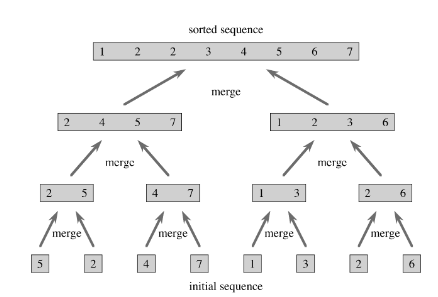
\includegraphics[width=6cm]{merge.png} 
        \caption{Mergesort diagram from \cite{cormen_introduction_2009}}
        \label{mrg}
    \end{figure}
    Mergesort has a time complexity of $O(nlog(n))$ in both the average and worst case, although constant factors can make it worse than Quicksort in practice. 
    Given the divide-and-conquer paradigm that Mergesort uses, it is a natural candidate for parallelization. Mergesort follows this paradigm as follows: First the input array (of size $n$) is recursively divided in two until there are $n$ single-element subarrays (divide). Each single-element array is trivially sorted (conquer). From there, the sorted subarrays are merged together, resulting in a single array that is equivalent to the input array but in sorted order (combine). Given the mechanics of the algorithm, there are two primary ways to parallelize Mergesort: (1) Parallelize the divide stage (i.e., the two recursive calls to the Mergesort procedure) and (2) Parallelize the combine stage (i.e., the Merge procedure). It is possible to implement either (1), (2), or both. According to \cite{cormen_introduction_2009}, only parallelizing the recursive calls to Mergesort will result in diminishing returns on performance as the number of processors grows to more than a few dozen. In order to efficiently scale up to hundreds of processors, parallelizing the merge procedure is necessary because it becomes the performance bottleneck.
    Our implementation of parallelized Mergesort is significantly based on \cite{radenski_mergesort}. The implementation parallelizes the recursive calls to Mergesort while implementing a serial merge procedure. There are a couple of reasons for this design decision. First, the HPC architecture we are using (the Case Western Reserve Markov cluster) has well under one hundred CPU cores per node. Thus, parallel Mergesort with only the divide stage parallelized theoretically scales well within this core-count range. Second, parallelizing the merge procedure proved to be difficult with OpenMP due to a lack of low-level control over threads. OpenMP is used to parallelize Mergesort by making use of OpenMP's parallel sections construct. A parallel sections region is created, and each recursive call to Mergesort is enclosed in its own parallel section. This allows OpenMP to spawn multiple threads that can execute the recursive calls in parallel. Nested parallelism is used so that each level of the recursion can spawn more threads (if they are available). The performance gains from this parallelism are significant as will be demonstrated in our Results section.
    
    % TODO @Jason add detail on your implementation and move before it Heapsort
    
    \subsection{Heapsort}
    The final sorting algorithm discussed here is Heapsort. Heapsort is yet another $O(nlog(n))$ comparison-based sorting algorithm. 
    It, along with the heap data structure, was invented in 1964. \cite{forsythe_algorithms_1964}
    Heapsort first turns the dataset into a max heap, which is a binary tree where each parent node is greater then its children. 
    This process, called \textit{heapification}, is an $O(n)$ algorithum. 
    Sorting is performed by repeatably popping the root node (the maximum value) and re-heapifying. 
    This procedure takes advantage of the binary tree structure, and is worst case $O(n log (n))$ overall.  \cite{cormen_introduction_2009}
    Unfortunately, Heapsort is a poor candidate for parallelization, as it does not divide or partition the input array into subarrays and depends on the root node being the absolute maximum. 
    
    \subsection{Quicksort}
    Quicksort is another $O(nlog(n))$ comparison-based sorting algorithm.
    Developed in 1961 \cite{hoare_algorithm_1961}, Quicksort is a partitioning sort that works by selecting a pivot element in an array and partitioning based on a comparison to the pivot, as shown in Figure \ref{qck}. 
    \begin{figure}[h]
        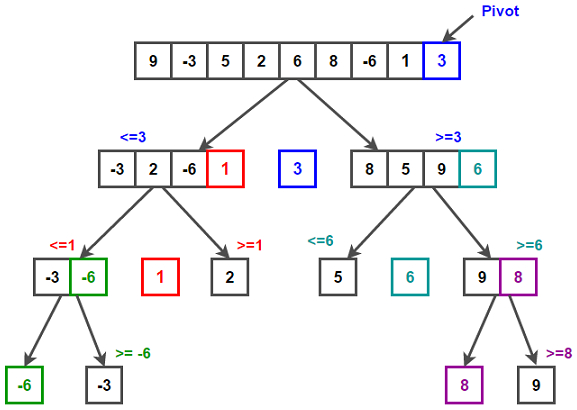
\includegraphics[width=6cm]{Quicksort.png} 
        \caption{Quicksort diagram. \href{https://www.techiedelight.com/quicksort/}{Source}}
        \label{qck}
    \end{figure}
    Similarly to Mergesort, Quicksort follows the divide-and-conquer paradigm. This makes Quicksort a naturally parallelizable sorting algorithm that can in theory achieve a significant performance increase with few modifications to its core logic. \cite{blelloch_programming_1996}
    This is because each subarray can be sorted independently, and this leads to speedup on parallel computers.
    The fundamental steps of Quicksort are as follows: The first step is to partition the array around a selected “pivot” point to produce two subarrays. These subarrays are then recursively sorted until the entire array of elements are in the correct order. Like Mergesort, there are two ways to parallelize Quicksort.
	We can parallelize the recursive calls to the Quicksort procedure, we can parallelize the Partition procedure, or both. To keep the design comparable to our Mergesort implementation, we opted to simply parallelize the recursive calls to Quicksort. OpenMP is used to parallelize Quicksort by making use of
	OpenMP task directives. In OpenMP, the task directive can tell OpenMP to dedicate a
	thread to a specific block of code labeled by the task. In this case, when the two subarrays are selected, each recursive call to the Quicksort method gets a dedicated OpenMP task initiated to create a parallel region of threads to be called later. This increases efficiency incredibly when allocating more and more OpenMP threads for Quicksort to use as is demonstrated in our Results section.
    \section{Methodology}
    For our project and experiment, we implemented our sorting algorithms in the C programming language. OpenMP \cite{openmp08} is used for achieving parallelization for our implementations of parallelized Mergesort and Quicksort.
    OpenMP facilitates multithreaded, shared-memory parallelism through the use of \textit{\#pragma} preprocessor directives in our C code.
	We ran our algorithms on Case Western Reserve University's HPC Markov cluster, which uses Intel Xeon x86\_64 processors. 

	The trials consisted of running our sorting algorithms on array sizes of $10,000$, $100,000$, $1,000,000$, $10,000,000$, $100,000,000$, and $1,000,000,000$ while using CPU core numbers of $1$, $2$, $4$, $8$, and $16$ for each array size. The execution times for each run of each array size/CPU count combination were collected and recorded in CSV files. From there, we analyzed the data in order to compare the performance and scalability of our sorting algorithms, producing several graphs in order to provide visuals for aiding in the analysis. The execution of our algorithms on the Markov cluster was achieved through the use of the Simple Linux Utility for Resource Management \cite{yoo_slurm_2003} (SLURM), which enables repeatable, large scale experiments to be performed with precisely configured resources. We wrote SLURM batch scripts that execute our sorting algorithms on Markov cluster compute nodes for each combination of array size and CPU count, and the execution times (measured in seconds) are returned in output files. The primary comparison is between Mergesort and Quicksort; however, Heapsort is included in our results as a reference serial algorithm. Heapsort is used as a sorting algorithm in the C standard library. It thus serves as an example of the performance that can be expected from calling a standard library sorting function, and so it is useful to see how its performance compares to our parallelized Mergesort and Quicksort.
    
    % TODO add more OMP detail here.  
    
    \section{Results}
    In this section, the results of each algorithm will be shown. 
    The main variable of interest is how much time each algorithm takes as a function of the length of the input array $n$.
    We begin with an individual discussion of Quicksort. 
    
    \subsection{Quicksort}
    There was great success with parallel Quicksort. 
    As a divide-and-conquer algorithm, it is a naturally parallel algorithum. 
    The results of this algorithum can be seen in Figure \ref{qck_per}. 
    \begin{figure}[h]
        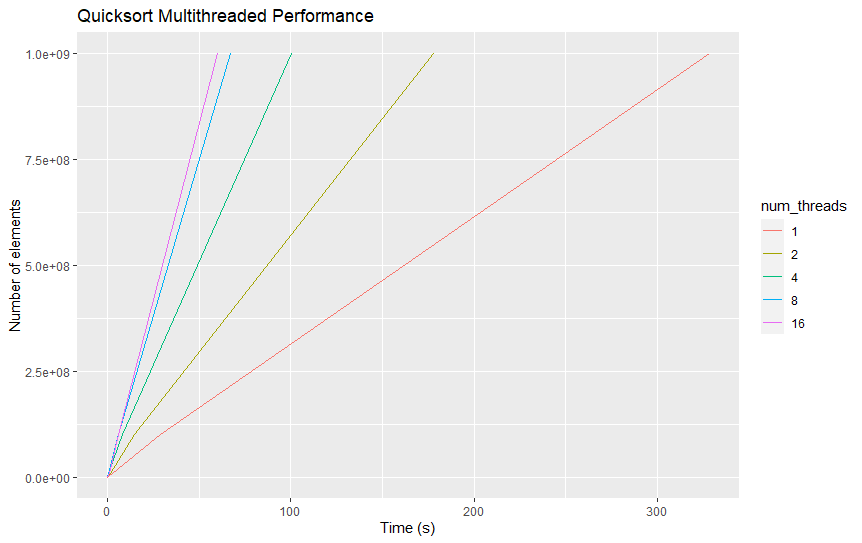
\includegraphics[width=9.25cm]{qs_mt.png} 
        \caption{Performance of Quicksort}
        \label{qck_per}
    \end{figure}
    
    %TODO add discussions on quicksort performance
    
    %TODO swap this section with next section

    \subsection{Heapsort}
    Heapsort proved to be purely sequential, as the core of the algorithm depends on universal array access in the current form. 
    The results of the nonparallel Heapsort are seen in Figure \ref{hs_per}. 
    \begin{figure}[h]
        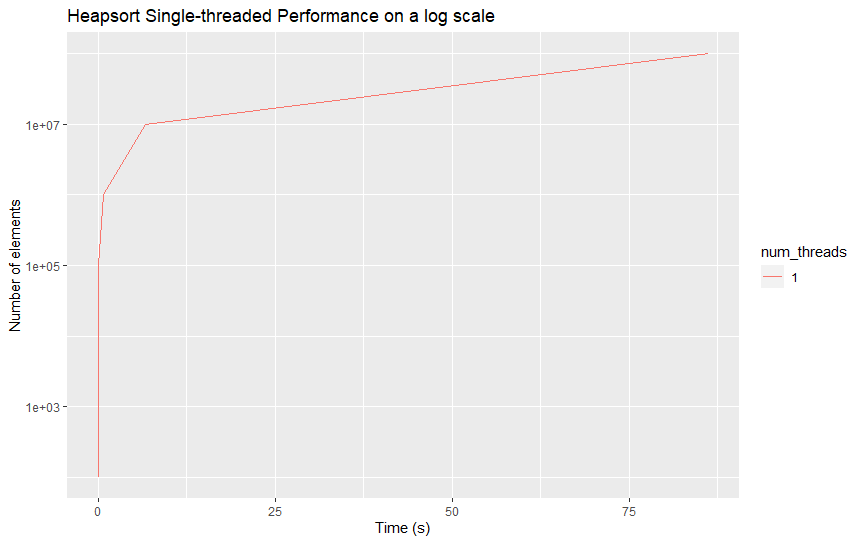
\includegraphics[width=9cm]{hs_per.png} 
        \caption{Performance of Heapsort}
        \label{hs_per}
    \end{figure}
    As Figure \ref{hs_per} shows, the performance of Heapsort becomes quite poor very rapidly. 
    Although in its current form, Heapsort cannot be parallelized, we present an alternative algorithm utilizing the core ideas of Heapsort in a parallel manner. 
    
    \begin{algorithm}
        \SetAlgoLined
        \KwResult{A sorted list }
        list $a$\;
        list $result$\;
        int $threads$\;
        let $lists$ be $a$ partitioned into $threads$\\
        \While{every list in lists is not empty }{
            \textbf{In Parallel}\;
            \hspace{0.5cm}$heapify$ each list\;
            $pop$ the largest element of all sub-heaps into $result$\;
            $re-heapify$ the heap that has been popped\;
        }
        \Return $result$
        \caption{Parallel-Heaps}
        \label{alg}
    \end{algorithm}
    Algorithm \ref{alg} presents a possibly parallel algorithm that utilizes the idea of Heapsort. 
    Essentially, the algorithm divides the array into many smaller heaps, each managed by a single thread. 
    This way, all heapification can be done in parallel, and the "max" item is selected from the number of heaps through a straightforward traversal of the roots of the sub-heaps. 
    However, this algorithum has several downsides. 
    One is that the end reheapification is still sequential; as by necessity, one heap must be popped, the algorithm must wait on the reheapification of that heap. 
    This heap will be smaller by a constant factor then the traditional, single-threaded Heapsort, however. 
    Therefore, $Parallel-Heaps$ will be at most a constant speedup for Heapsort.
    
    $Parallel-Heaps$ was not implemented in this study, as it is not possible to do with the OpenMP framework; such a method would require POSIX threads. 
    For the sake of comparison, this algorithm was thus excluded. 
    Further investigation of this $Parallel-Heaps$ algorithm is a topic for further study.  
    \subsection{Mergesort}
    As with Quicksort, Mergesort proved to be naturally parallel. 
    The results of parallel Mergesort can be seen in Figure \ref{ms_per}
    \begin{figure}[h]
        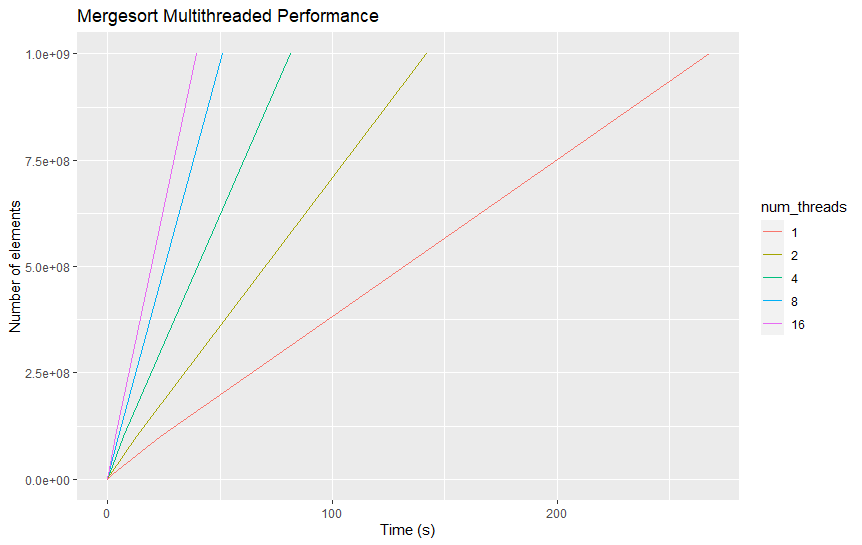
\includegraphics[width=9cm]{ms_per.png} 
        \caption{Performance of Mergesort}
        \label{ms_per}
    \end{figure}
    %TODO add mergesort implementation details
    
    
    
    \subsection{Shellsort}
    
    For our analysis, we attempted to implement an additional algorithm, Shellsort. We were unsuccessful. We include Shellsort here, however, for completeness and for the Case Western Reserve University HPC developer that may find themselves wondering about Shellsort's parallel implementation. Shellsort is an seen to be a generalization of a more elementary sorting algorithm, Insertionsort, and uses the Insertionsort algorithm in its subroutines. Because of Insertionsort's dependence on access to the entire input array per swap movement, all Insertionsort swaps must be done in serial or risk a data race, which would jepordize the sort's integrity. For this reason, Insertionsort is nonparallelizable, yet performant in small array size scenarios. Shellsort, however, improves on Insertionsort's design by incorporating a divide and conquer strategy. In particular, Shellsort begins by in-place Insertionsorting small, distant subsets of the input array before peforming Insertionsort on the whole resulting array. This final Insertionsort is done because Insertionsort has fantastic $O(N)$ performance for almost-sorted arrays.  Since all Shellsort's subroutines contribute to advancing the array's state in regards to reaching an optimal setup for the final Insertionsort call and that Shellsort's final serial Insertionsort call on the whole array will inevitably fix any gaps the setup stage missed, Shellsort is a natural candidate to parallelization. A perfunctory parallelization attempt, like the one attemped in the appendix, then can implemented by partitioning an input array into disjoint blocks, having sorting them each sorted in parallel with an OMP recursive call to Shellsort, and then running Shellsort in serial on the result of all those in-place recursive sorts. Note Shellsort's particular potential success in giving each CPU of the OMP tasks significant work to do per unit parallel time. This is what would contribute to such an Implentations potential average span of $O(logn)$. Unfortunately, such an implementation was not found to be possible for us at this time, due to issues with redistrubuting the number of active cores in a loop using the OpenMP framework.  
    
    \subsection{Comparative Results}
    Results are compared in a few different ways. 
    One is to hold the number of threads constant, and plot the performance of each algorithm, as in Figure \ref{msqshs}, which shows that Heapsort, which is not paralleized, proves to be much worse then either Quicksort or Mergesort.
    \begin{figure}
        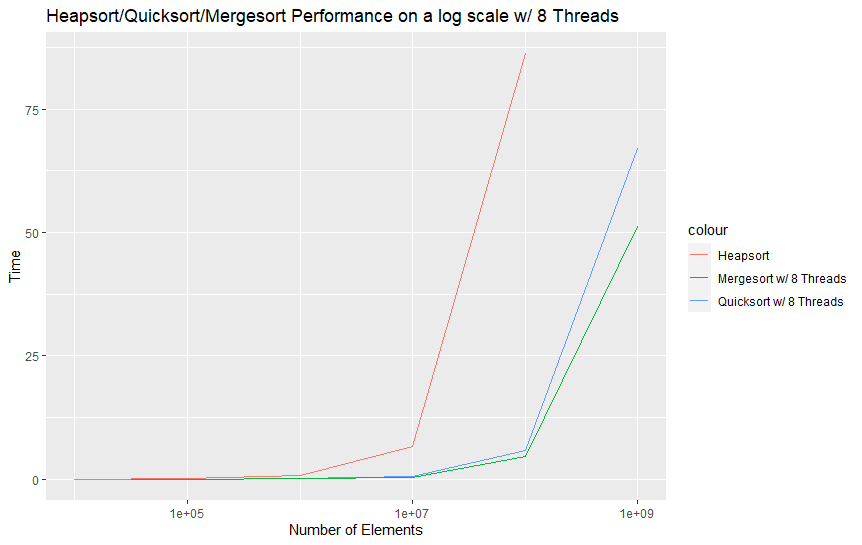
\includegraphics[width=9.25cm]{mshsqs.png} 
        \caption{Comparative Performance with 8 threads}
        \label{msqshs}
    \end{figure}
    %TODO Add deets
    Additionally, it is useful to compare results on a single array size with multiple threads. 
    This can be seen for $10^6$ elements in Figure \ref{1e5}
    \begin{figure}
        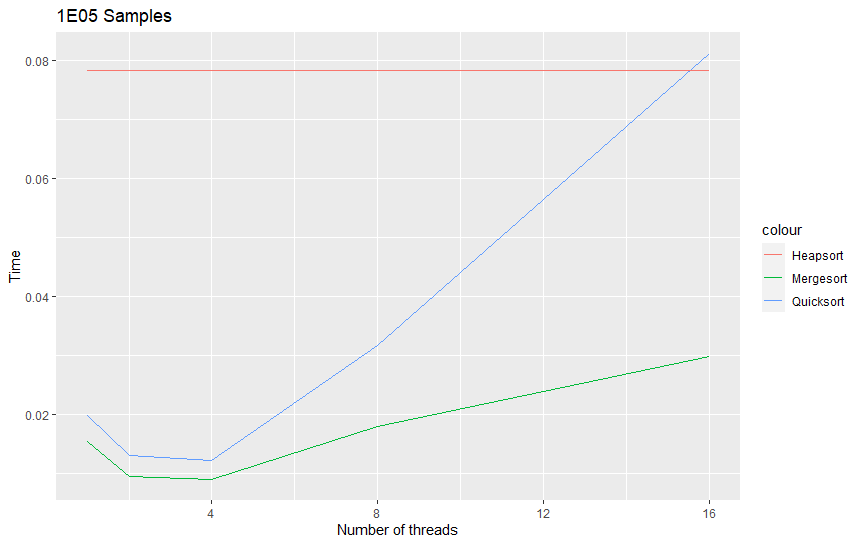
\includegraphics[width=9cm]{1e5.png} 
        \caption{Comparative Performance with for $10^4$ elements}
        \label{1e5}
    \end{figure}
    Interestingly, the performance of Quicksort appears to worsen with the number of threads more then Mergesort; this suggests significant overhead introduced by parallelization. 
    However, this effect goes away with an increase in the number of elements, as in Figure \ref{1e8}. 
    \begin{figure}
        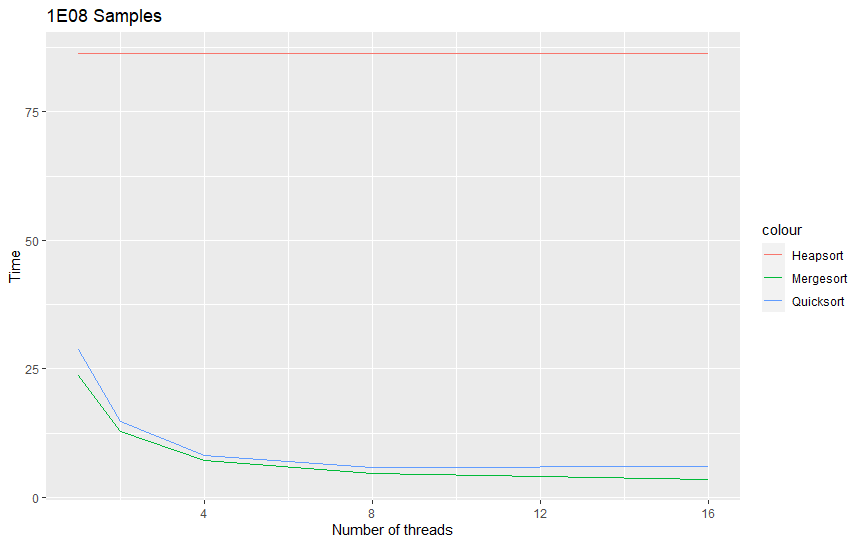
\includegraphics[width=9cm]{1e8.png} 
        \caption{Comparative Performance with for $10^7$ elements}
        \label{1e8}
    \end{figure}
    
    This suggests that there is significant overhead with smaller array sizes, but this is overcome by efficeicny gains on larger array sizes. 
    \section{Conclusion}
    % TODO these are what we expect to see...
    As expected, the three $O(n log(n))$ algorithms perform better then Insertion sort. 
    Due to the more parallel nature of Quicksort and Mergesort, these algorithms benefit more from parallization then the more sequential Heapsort. 
    This is because the divide and conquer strategy is inherently more parallel, which should be taken into account when developing new algorithms to be run on parallel and distributed computing platforms. 
    % TODO further findings from implementation
    \bibliography{ref.bib}
    \bibliographystyle{ieeetran}
    \appendix
	All of our code and data can be found in our GitHub repo \href{https://github.com/causeyc/csds438_sorting}{here}. Our implementation of parallel Mergesort is located in mergesort/merge$\_$sort$\_$OpenMP.c. The parallel Quicksort implementation is in quicksort/quicksortOMP.c. Our serial Heapsort implementation is located in heapsort/heapsort.c. In order to run the experiment, clone the repo into a location on Case Western's HPC Markov cluster. From there, run the SLURM batch scripts. The first is \textbf{sorting.slurm} and is located in mergesort/. This script runs parallel Mergesort on a compute node on all combinations of array sizes and CPU core numbers (as explained in the main part of the paper). Once finished, an output SLURM file will be produced that contains the execution times of the sorts. \textit{Mutatis mutandis} for Quicksort (the batch script is called \textbf{qs-job.slurm} and is located in quicksort/). CSV files that we manually created from the data produced from our SLURM jobs are located in mergesort/ and quicksort/ and are called "MergeSort Data.csv" and "project.csv", respectively.
    % TODO slap the code in here
\end{document}
